\section{Testing and evaluation}

%TODO:  * rewrite the 10c thing and introcude it at the end the sampling section
%       * Re-organized all tasting explanation in the testing section, with a general introduction to it based on the diagram.
%       * Delete table about training set and remove all mentions of it.
%       * re-factor NL section

%THE TRAINIG SET IS NOT REALLY RELEVANT TO THIS CHAPTER, CONSIDER REMOVING MENTIONS OF IT AND ONLY SHOW TESTS AGAINST THE TESTING SET.
In this next section, we are going to evaluate the performance of the PassGAN system, as well as give a brief overview of our methodology and the experimental setup.

\subsection{Experimental setup}
Both training of the GAN and testing were carried out on a Linux machine running Debian stretch, equipped with a GTX 1070 graphics card, an i5-2500 CPU and 8 GB of system memory. 
With this card, training of PassGAN took roughly twelve hours.
PassGAN was run on Python 2.7, running Tensorflow 1.12.0.%\\

For testing we used the latest stable version of HashCat as of this writing (version 5.1.0). %and we observed a peak speed between 850 and 860MH/s (for reference, 1MH/s is equivalent to 1 million candidate passwords hashed and compared per second) %Reference  %The definition of MH is probably wrong

Figure \ref{fig:testing_flowchart} below illustrates our overall process, which is divided in two Phases: 
\begin{itemize}
    \item A Training Phase, in which we train PassGAN on a given dataset and sample password candidates from the trained model.
    \item A Testing Phase, in which we use HashCat to try and crack a subset of the Passwords in the libero leak.
\end{itemize}

\begin{figure}[H]
\centering
    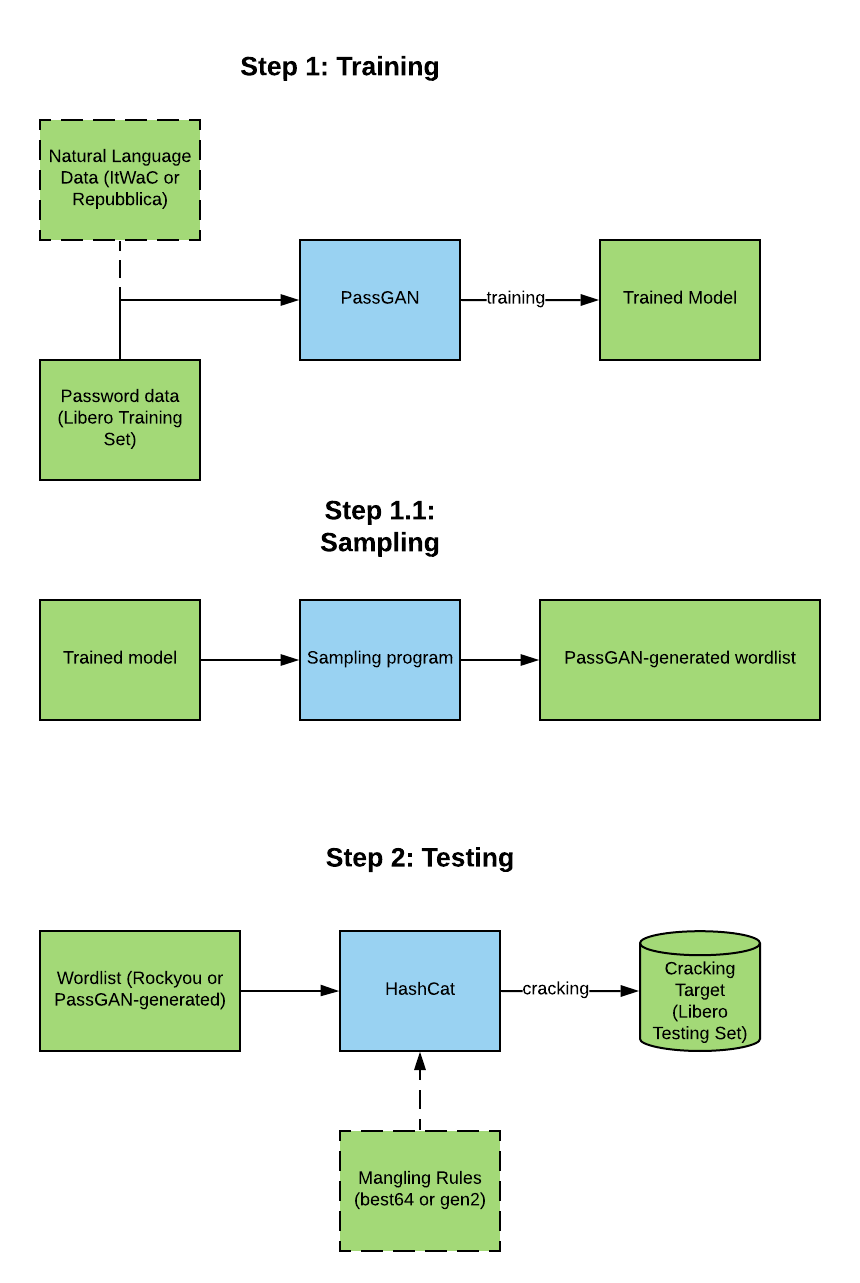
\includegraphics[scale=0.8]{figures/testing_flowchart.png}
    \caption{A diagram illustrating out general workflow for evaluating PassGAN, including Training and Testing}
    \label{fig:testing_flowchart}
\end{figure}    

\subsection{Training and testing the PassGAN system}
In order to train PassGAN we took the plain text passwords from the libero leak (667,714 passwords) and split them into two groups: 80\% of the passwords went into our Training Set, while the remaining 20\% of passwords went in the Testing set: The Training set is used to train PassGAN as can be seen in Step 1 of figure \ref{fig:testing_flowchart}, while the passwords in the Testing set are hashed with MD5 to serve as a cracking target for HashCat (this process can also be observed in the code snippet at the end of the previous section).

PassGAN can additionaly be trained on Natural Language data, shown in a dotted box in figure \ref{fig:testing_flowchart}; elements shown within a dottet box are considered optional, they can be included or not. Natural Language data will be further discussed in secion \ref{subsec:nl-testing}.

Once PassGAN is done training with a given dataset, it produces a training model that can be used to generate candidate passwords via sampling (Step 1.1 in the figure). This sample of candidate password will be the PassGAN wordlist used with Hashcat when testing, and we can choose to generate more or less candidate passwords when sampling: the tests listed in table \ref{tab:test-set} use a wordlist of 1 million password candidates, while tables \ref{tab:passgan-big} and \ref{tab:nl-results} use a wordlist of roughtly 14 million password candidates.



%In order to train the PassGAN system, we extracted the plain text passwords from the original file (which was formatted in JSON as it contained personal information beyond just the emails and passwords of the users), and split it up in two sets: a training set containing 80\% of the passwords (534,171 entries) and a testing set containing 20\% of the passwords (133,542 entries).
%We used the model trained on the bigger set to generate 1 million samples from PassGAN, that then served as the basis from our initial testing.

Below is an example of samples that were produced by PassGAN at the very end of training: %Maybe i should take a sample from the last checkpoint instead?
\begin{verbatim}
22052906    mariamuna   �iaup63     poldetta53
001178      04051987    topolapa    aenara
rotsanera   princone    fadyreda21  giugki
dimonepa72  12orlomon   deb57828    belnabola
marcanalla  ACADCNA�N   leegenniki  vicaletto
\end{verbatim}

%Give a small eexample of one or two particular words and words in italian that resemble them.
What we found particularly interesting was that while the samples showed the typical patterns exhibited by user-generated Passwords (numbers appended or pre-pended to words, so-called leet speak etc..), a majority of them also seemed to mimic Italian words and phrases: most of these words were meaningless, but nonetheless we speculated that the GAN might be trying to \enquote{learn} Italian as a side-effect of generating samples close to the input data distribution.
As an example the string \texttt{vicaletto} resemble the italian word \enquote{vicoletto} meaning \enquote{a narrow street}, while the string \texttt{princone} sounds vaguely like the italian word for pickaxe \enquote{piccone}. 
\subsection{Testing the PassGAN system (Placeholder)}
During our testing we tried to follow the same sort of methodology that Hitaj et al.\cite{PassGAN} used in their paper: as such, in our testing we used a subset of both our training  and our testing set, composed of passwords with a length of 10 characters or less. This was done in order to focus the scope of PassGAN, as during training we set the sequence length to 10.\\ %Bullshit you just wanna give yourself a leg up. %MAYBE the oassgan ppl trained the GAN on a 10c datasets as well? maybe i should re-train to test this.
We believe this sub-set of ten-character is still representative of the whole set, as the vast majority of passwords in the Libero set are 10 characters or less: 461,442 (86.38\%) in the Training set, and 111,994 (83.86\%) in the Testing set. 

In order to test the performance of PassGAN, we compared it with other wordlists and rules commonly used in rule-based password crackers: Specifically we chose \emph{RockYou} as our wordlist, alongside \emph{best64} and \emph{generated2} as our rules; All of them were chosen because they were also used by Hitaj et al.\cite{PassGAN}.
The RockYou wordlist contains more than 14 million strings, all of which come from various data breaches that have been compiled into one resource; it contains password of varying length and complexity, and as such should provide a good performance baseline for rule-based crackers. The best64 rules file contains around 70 mangling rules, while the genrated2 rules file contains more than 65,000. 
Finally in order to test the output of PassGAN we used a wordlist containing one million samples generated by the model we trained earlier.
A further reason why we chose to use the RockYou wordlist and the two rule sets described above is that they are widely used, and understood to be among the more efficient wordlists available to an attacker; we believe that they demonstrate rather well what rule-based password crackers can do without further language specific optimizations such as those that PassGAN provides.

The tables below will illustrate the results of our tests, performed on both the Training set and the Testing set using the wordlists and rules described above. To clarify, we decided early on to use mangling rules also when testing password samples from PasGAN, since they greatly increased the number of passwords found. 

Hashcat's default behaviour is to cache passwords found during an attack in what the Hashcat manual calls a \emph{potfile}, so that if an attacker chooses to approach the target using a different wordlist or a different set of rules, no time is wasted cracking passwords that were already found previously; because using different rule sets can greatly affect the efficiency of cracking, this form of caching allow an attacker to crack more passwords by combining different approaches.
In order to test the performance of each combination separately, we disabled caching of cracked passwords between cracking attempts: this allowed us to evaluate the performance of different combination of wordlists and rules singularly, but it also translates in a lower overall number of passwords found; tables \ref{tab:test-set}, \ref{tab:train-set} and \ref{tab:passgan-big} show show tests done with caching disabled, while the figures obtainable with caching will be mentioned at the very end of this section. 

\begin{table}[H]
\begin{tabular}{|l|c|c|c|}
\hline
\textbf{\emph{Wordlist/Ruleset}} & \textbf{-} & \textbf{Best64} & \textbf{Gen2} \\ \hline
\textbf{Rockyou}          & 19,215 (23.78\%) & 30,170 (37.33\%) & 59,134 (73.18\%) \\ \hline
\textbf{PassGAN}          & 4,637 (5.74\%) & 11,053 (13.68\%) & 34,896 (43.18\%) \\ \hline
\end{tabular}}
\caption{Number of passwords found in the Testing set}
\label{tab:test-set}
\wfill
\hfill

\begin{tabular}{|l|c|c|c|}
\hline
\textbf{\emph{Wordlist/Ruleset}} & \textbf{-} & \textbf{Best64} & \textbf{Gen2} \\ \hline
\textbf{Rockyou}          & 70,550 (25.36\%) & 115,339 (41,47\%) & 202,624 (72.85\%) \\ \hline
\textbf{PassGAN}          & 15,924 (5.72\%) & 40,659 (14.62\%) &  134,114 (48.22\%) \\ \hline
\end{tabular}}
\caption{Number of passwords found in the Training set}
\label{tab:train-set}
\end{table}

As table \ref{tab:test-set} and \ref{tab:train-set} show, the relative amount of password found with each technique is roughly consistent between the two sets.
One point is immediately evident, and that is that PassGAN performs rather poorly in comparison: we attributed this shortcoming to two main factors: firstly the size of the wordlist generated by PassGAN, which is 1 million entries as opposed to the 14+ million entries of RockYou, the second factor is the quality of the PassGAN wordlist; both of these factors play into each other, because while the rules provide great advantages in terms of password found, ultimately they just modify the entries in the wordlist. Thus we might say that the whole system is limited by the capabilities of the wordlist that is used.

In order to test this hypothesis we used our existing PassGAN model to generate a bigger wordlist with as many entries as as RockYou, and performed a second test on the Testing password set:
\begin{table}[H]
\centering    
\begin{tabular}{|l|c|c|c|}
\hline
\textbf{\emph{Wordlist/Ruleset}} & \textbf{-} & \textbf{Best64} & \textbf{Gen2} \\ \hline %First row is wrong, you copied from Training. 
\textbf{Rockyou}          & 19,215 (23.78\%) & 30,170 (37.33\%) & 59,134 (73.18\%) \\ \hline
\textbf{PassGAN (14 million entries)}          &  10,735 (13.28\%) & 20,638 (25.54\%) & 48,751 (60.33\%) \\ \hline
\end{tabular}}
\caption{Number of passwords found in the testing set with a bigger PassGAN wordlist} 
\label{tab:passgan-big}
\end{table}

As table \ref{tab:passgan-big} shows, PassGAN found roughly 15\% more passwords when using a bigger wordlist: this leads us to believe that wordlist size and quality does constitute a performance bottle-neck. It should be also noted that when compared with the original, 1 million string wordlist, we found a significant 40\% overlap in the strings that were generated. Addressing the problem of quality of the wordlist, we speculate that one of the reasons for the gap in efficiency between PassGAN and RockYou might be the fact that the strings generated by PassGAN don't follow grammatical rules, and this might hinder the efficacy of the base wordlist. Mangling rules help greatly in finding passwords, but ultimately they are patterns applied to the base wordlist entries: if the base wordlist is less efective becasue it does not follow grammatical rules, the combined efficiency will go down.
This hypothesis will be proven wrong in section \label{subsec:nl-testing}.

When running rockyou and PassGAN sequentially on the testing set using the gen2 ruleset, we get the overall best results with 79.01\% of password matched (63,847 passwords): PassGAN found an additional 4,713 passwords that were not matched by RockYou, consisting of mostly Proper names and italian words.

\subsection{Natural language corpora} \label{subsec:nl-testing}
%Find a more reader-friendly explanation for grammatical correctness, especially at the beginning  when defining the goal.
Our next step was to include natural language data in the input and re-train the model, in the hope that this new input data would help the system generate more grammatically correct strings and thus improve the number of passwords matched.

%Talk about how the words in the corpora are sorted and how you scrambled them.%Talk about how the words in the corpora are sorted and how you scrambled them.%Talk about how the words in the corpora are sorted and how you scrambled them.%Talk about how the words in the corpora are sorted and how you scrambled them.%Talk about how the words in the corpora are sorted and how you scrambled them.%Talk about how the words in the corpora are sorted and how you scrambled them.%Talk about how the words in the corpora are sorted and how you scrambled them.
For this purpose we have chosen two different corpora of Italian Natural Language samples: 
\begin{itemize}
    \item The Repubblica corpus: A corpus of words extracted from the italian newspaper "Repubblica", taken from articles published between 1985 and 2000 (roughly 380 million words).\cite{repubblica_corpus}
    \item The ItWaC corpus: A large 2 billion word corpus obtained by crawling internet sites under the \texttt{.it} domain. \cite{itwac_corpus}.  
\end{itemize}
%You can increase the number of guesses by generating more samples and increasing the size of the wordlist, though there might be diminishing returns at some point.
%The nice thing about PassGAN is that you have theoretically infinite wordlists, even if the quality might be up and down.
Both corpora were generated using the NoSketch Engine online tool \cite{nosketch_engine}, and we decided to sample two dataset from each corpus with the same number of entries as the libero password set. This was done to ease the process of organizing data for training PassGAN, and also because we were concerned about the impact that different ratios of password data to natural language might have on the resulting model.
Previous research \cite{Melicher2016} has suggested that introducing Natural Language data into a system trained on passwords tends to generate a lot of noise during training, and our results turned out to be in line with that paper.

The data preparation process for the Natural Language datasets was very similar to what we did for the libero set, we divided our datasets into 80\%-20\% subsets: while this was not strictly necessary since we did not intend to crack the natural language datasets (that was why we originally held back 20\% or our password data), we went ahead anyway in case we needed to do that later. 

In order to test the impact of a large quantity of natural language data, we compiled two wordlists for each corpus for a total of four: for each corpus we had one shorter wordlist and one longer one.
The shorter wordlists contained all of the password data we used in our first model plus 50\% of the respective NL corpus, while the longer ones contained all of the password data and all of the NL data for their corpus.
The results of our tests on all four wordlists are shown in table \ref{tab:nl-results} below. It should be also noted that in order to maximize the number of passwords found, all tests where run using the Gen2 rule set and using the same number of PassGAN samples as table \ref{tab:passgan-big} for this reason the numbers shown in the following table should be mostly compared with table \ref{tab:passgan-big}.

Our hypothesis was that we might see a decrease in model performance in the second case, since the full NL datasets contains as much data as the password one and this might lead to noise, resulting in a model with less focus on generating passowrds as opposed to generating NL samples. While that is technically true, overall table \ref{tab:nl-results} shows that the introduction of NL data does not seem to have any positive impact of cracking performance.

% Table \ref{tab:nl-results} below shows the results of our tests for both datasets: the entries labelled with 50\% are composed of the 80\% of the libero set and 50\% of the natural language data from that source, while the other two entries are the results of PassGAN when trained on 80\% of the libero set and all of the natural language data instead. All tests were persormed using the generated2 ruleset.\\
% After re-training PassGAN using natural language samples with the process outlines above, we find that the inclusion of this new NL data does not seem to have much of an effect of the cracking performance of PassGAN;
\begin{table}[H]
\centering
\begin{tabular}{|l|l|}
\hline
\textbf{Repubblica 50\%} & 51,232 (63.40\%) \\ \hline
\textbf{Repubblica 100\%} & 48,651 (60.20\%)  \\ \hline
\textbf{ItwaC 50\%} & 50,133 (62.04\%)  \\ \hline
\textbf{ItWaC 100\%} & 47,646 (58.96\%)  \\ \hline
\end{tabular}
\caption{Number of passwords found in the Testing set using PassGAN trained on passwords and Natural Language data}
\label{tab:nl-results}
\end{table}

As we can see the results of training with natural language data are very similar to just using PassGAN+gen2 as shown in table \ref{tab:passgan-big}; there is a slight improvement of 2-3\% when using the datasets containing 50\% of language data, but we do not believe it is a significant change. This result seems to be in line with Melicher et al.\cite{Melicher2016}, and it seems to show us that natural language data does not have much of an impact on the output of PassGAN. 
\newpage
If we take a random sample from the Repubblica 50\% set, the one that performed the best even if marginally so, we can see that there has not been a substantial improvement in the grammatical correctness of the entries:
\begin{verbatim}
c3b243dc    fetemanio   carcilla    RATS1203
valentto    itefis82    carmoinx    gip1904
sederonco   elestarsia  220689      Q�unkYYTx84
n!utelo     kedea       Colpudari   rich1770
aletsa      simoshero   gidni12     1uva1[78
\end{verbatim}    

The words that PassGAN are still meaningless and does not seem to have a higher degree of grammatical correctness, the only change we have been able to observe is in the fact that more strings seem to be composed of letters exclusively.

This does not discredit the use of Natural language as a whole, but points us toward the fact that natural language generation and password generation are two different workloads that may not be accomplished well with the same machine learning system: it seems that introducing Natural Language data into PassGAN simply adds noise to the system and does not contribute to the system's performance.
The results in table \ref{tab:nl-results} and the effectiveness of mangling rules as a cracking tool also hint at the idea that user-generated passwords may be defined by their patterns more than by their language of origin. 
